% ========================================================================
% Monetary Policy Research Proposal — Beamer Presentation
% Eileen Zhang | Academic Economics/Finance
% ========================================================================
\documentclass[aspectratio=169, 11pt]{beamer}

% ── Packages ─────────────────────────────────────────────────────────────
\usepackage[fontset=fandol]{ctex}
\usepackage{amsmath, amssymb, mathtools}
\usepackage{booktabs, tabularx}
\usepackage{graphicx}
\usepackage{xcolor}
\usepackage{tikz}
\usetikzlibrary{arrows.meta, positioning, shapes.geometric, calc, fit}
\usepackage[most]{tcolorbox}
\usepackage{ragged2e}
\usepackage{hyperref}

% ── Theme ────────────────────────────────────────────────────────────────
\usetheme{Madrid}
\usecolortheme{dolphin}
\usefonttheme{professionalfonts}
\usefonttheme{serif}
\justifying

% ── Colors: Academic Navy + Burgundy ─────────────────────────────────────
\definecolor{myblue}{HTML}{0B1F3A}
\definecolor{myaccent}{HTML}{8B1A1A}
\definecolor{mygreen}{HTML}{1B5E20}
\definecolor{mygray}{HTML}{F0F2F6}

\setbeamercolor{frametitle}{bg=myblue, fg=white}
\setbeamercolor{structure}{fg=myblue}
\setbeamercolor{block title}{bg=myblue!90, fg=white}
\setbeamercolor{block body}{bg=myblue!8}
\setbeamercolor{alerted text}{fg=myaccent}
\setbeamercolor{title}{fg=white}
\setbeamercolor{subtitle}{fg=white!85}
\setbeamercolor{author}{fg=white!90}
\setbeamercolor{institute}{fg=white!75}
\setbeamercolor{date}{fg=white!75}
\setbeamercolor{titlelike}{bg=myblue, fg=white}

% ── tcolorbox blocks ─────────────────────────────────────────────────────
\tcbset{
  blocksty/.style={
    boxrule=0.4pt, arc=1.5pt,
    top=3pt, bottom=3pt, left=5pt, right=5pt,
    fonttitle=\bfseries\small, before upper={\small}, valign=top,
  }
}
\newtcolorbox{fblock}[2][]{blocksty, colback=myblue!8, colframe=myblue!85,
  coltitle=white, title={#2}, height=#1}
\newtcolorbox{falertblock}[2][]{blocksty, colback=myaccent!8, colframe=myaccent!80,
  coltitle=white, title={#2}, height=#1}
\newtcolorbox{ablock}[1]{blocksty, colback=myblue!8, colframe=myblue!85,
  coltitle=white, title={#1}}
\newtcolorbox{aalertblock}[1]{blocksty, colback=myaccent!8, colframe=myaccent!80,
  coltitle=white, title={#1}}
\newtcolorbox{agreenblock}[1]{blocksty, colback=mygreen!8, colframe=mygreen!80,
  coltitle=white, title={#1}}

% ── Navigation: Use Madrid's built-in infolines footer ───────────────────
\setbeamertemplate{navigation symbols}{}
% Madrid theme already provides a clean infolines footer with section + page info

% ── Auto section title pages ────────────────────────────────────────────
\AtBeginSection[]{
  \begin{frame}[plain]
    \vfill
    \centering
    \begin{beamercolorbox}[sep=12pt,center,rounded=true,shadow=true]{title}
      \usebeamerfont{title}\Large\insertsectionhead\par
    \end{beamercolorbox}
    \vfill
  \end{frame}
}

% ── Fonts ─────────────────────────────────────────────────────────────────
\setbeamerfont{title}{size=\LARGE, series=\bfseries}
\setbeamerfont{subtitle}{size=\large}
\setbeamerfont{frametitle}{size=\large, series=\bfseries}
\setbeamerfont{block title}{size=\normalsize, series=\bfseries}
\setbeamerfont{footnote}{size=\tiny}

\hypersetup{hidelinks}

% ── Metadata ─────────────────────────────────────────────────────────────
\title[Monetary Policy \& Asset Prices]{Monetary Policy Announcements, \\ Asset Prices, and Portfolio Reallocation}
\subtitle{A Research Proposal}
\author[E. Zhang]{Eileen Zhang}
\institute{Department of Finance}
\date{August 2026}

% ========================================================================
\begin{document}

% ── Title Slide ──────────────────────────────────────────────────────────
\begin{frame}[plain]
  \titlepage
\end{frame}

% ── Outline ──────────────────────────────────────────────────────────────
\begin{frame}{Outline}
  \tableofcontents
\end{frame}

% ========================================================================
\section{Background \& Rationale}
% ========================================================================

\begin{frame}{The 2022--2025 Tightening Cycle: A Stress Test}
  \begin{columns}[T]
    \column{0.55\textwidth}
    \begin{ablock}{Unprecedented in Four Decades}
      \begin{itemize}
        \item Fed funds rate: $0.25\% \to 5.50\%$ in 18 months
        \item \alert{Simultaneous} selloffs in equities and bonds
        \item 60/40 portfolio posted $-17\%$ in 2022
        \item Negative stock-bond correlation \alert{broke down}
      \end{itemize}
    \end{ablock}

    \column{0.42\textwidth}
    \begin{aalertblock}{Key Question}
      Does FOMC communication contain \textbf{incremental information} \\
      beyond the rate decision itself, \\
      that drives asset price movements?
    \end{aalertblock}
  \end{columns}
\end{frame}

\begin{frame}{Three Gaps in the Literature}
  \begin{columns}[T]
    \column{0.31\textwidth}
    \begin{fblock}[4.2cm]{Methodological Gap}
      \footnotesize
      Kuttner (2001) $\to$ JK (2020) $\to$ Bauer-Swanson (2023): \\
      identification evolved, but \alert{rarely integrated} with NLP-based \\
      sentiment analysis.
    \end{fblock}

    \column{0.31\textwidth}
    \begin{falertblock}[4.2cm]{Empirical Gap}
      \footnotesize
      2022--2025 cycle lacks systematic study: \\
      rapid hikes, QT, inflation shocks, and \\
      \alert{shifted communication regime} \\
      are poorly understood.
    \end{falertblock}

    \column{0.31\textwidth}
    \begin{fblock}[4.2cm]{Measurement Gap}
      \footnotesize
      Dictionary-based sentiment (LM, CB) is coarse; FinBERT is available but \alert{lack of large-scale \\
      reproducible pipeline} \\
      for FOMC statements.
    \end{fblock}
  \end{columns}

  \vspace{0.4em}
  \begin{center}
    \small This proposal addresses all three gaps simultaneously.
  \end{center}
\end{frame}

% ========================================================================
\section{Research Aim \& Objectives}
% ========================================================================

\begin{frame}{Research Aim}
  \begin{center}
    \begin{tcolorbox}[blocksty, colback=myblue!8, colframe=myblue!85,
      coltitle=white, width=0.92\textwidth,
      title={Research Aim}]
      \normalsize
      To quantify the \textbf{incremental information content} of FOMC \\
      communication beyond policy rate surprises, and to examine its \\
      \textbf{differential transmission} across asset classes and \\
      \textbf{regime-dependent} effects on portfolio reallocation.
    \end{tcolorbox}
  \end{center}

  \vspace{0.3em}
  \begin{center}
    \small Contributing to: monetary economics $\cdot$ central bank communication $\cdot$ asset pricing
  \end{center}
\end{frame}

\begin{frame}{Four Objectives \& Four Hypotheses}
  \centering
  \footnotesize
  \begin{tabularx}{\textwidth}{>{\bfseries}l X l}
    \toprule
    & \textbf{Objective} & \textbf{Hypothesis} \\
    \midrule
    O1 & Measure sentiment-surprise overlap & $H_1$: $0 < \beta < 1$ \\
    O2 & Test incremental explanatory power & $H_2$: $\beta_2 \neq 0$ \\
    O3 & Map sentiment to structural shocks & $H_3$: $|\gamma_2| > |\gamma_1|$ \\
    O4 & Identify regime-dependent effects & $H_4$: $\beta_3 \neq 0$ \\
    \bottomrule
  \end{tabularx}

  \vspace{0.5em}
  \begin{itemize}
    \item<1-> \textbf{O1:} Is sentiment correlated with but distinct from rate surprise?
    \item<2-> \textbf{O2:} Does sentiment explain asset returns \emph{after} controlling for rates?
    \item<3-> \textbf{O3:} Does sentiment capture the \emph{information} shock, not just policy shock?
    \item<4-> \textbf{O4:} Are effects stronger during forward guidance / ZLB periods?
  \end{itemize}
\end{frame}

% ========================================================================
\section{Literature Review \& Hypotheses}
% ========================================================================

\begin{frame}{Monetary Policy Surprise: Identification Evolution}
  \centering
  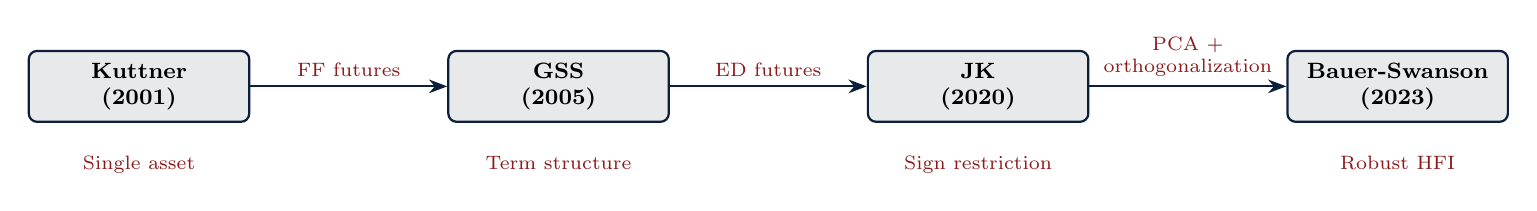
\begin{tikzpicture}[
    node distance=1.2cm,
    box/.style={rectangle, rounded corners=3pt, draw=myblue, thick,
      fill=myblue!10, minimum width=2.8cm, minimum height=0.9cm, font=\footnotesize\bfseries, align=center},
    arr/.style={-Stealth, thick, myblue},
    note/.style={font=\scriptsize, text=myaccent, align=center}
  ]
    \node[box] (k) {Kuttner\\(2001)};
    \node[box, right=2.5cm of k] (gss) {GSS\\(2005)};
    \node[box, right=2.5cm of gss] (jk) {JK\\(2020)};
    \node[box, right=2.5cm of jk] (bs) {Bauer-Swanson\\(2023)};

    \draw[arr] (k) -- node[above, note] {FF futures} (gss);
    \draw[arr] (gss) -- node[above, note] {ED futures} (jk);
    \draw[arr] (jk) -- node[above, note] {PCA +\\orthogonalization} (bs);

    \node[below=0.3cm of k, note] {Single asset};
    \node[below=0.3cm of gss, note] {Term structure};
    \node[below=0.3cm of jk, note] {Sign restriction};
    \node[below=0.3cm of bs, note] {Robust HFI};
  \end{tikzpicture}

  \vspace{0.5em}
  \begin{itemize}
    \item \textbf{Key insight:} identification moved from \emph{single-asset} to \emph{multi-asset PCA}, addressing the ``information effect'' (Nakamura \& Steinsson, 2018)
    \item \alert{Gap:} None of these integrate \textbf{textual sentiment} as a separate shock
  \end{itemize}
\end{frame}

\begin{frame}{Central Bank Communication: NLP Evolution}
  \begin{columns}[T]
    \column{0.48\textwidth}
    \begin{ablock}{Dictionary-Based}
      \begin{itemize}
        \item Loughran \& McDonald (2011): finance-specific word lists
        \item Apel \& Blix (2014): CB hawkish/dovish dictionary
        \item \alert{Limitation:} no context, no negation, no sarcasm
      \end{itemize}
    \end{ablock}

    \column{0.48\textwidth}
    \begin{aalertblock}{ML-Based}
      \begin{itemize}
        \item FinBERT (Araci, 2019): fine-tuned BERT
        \item Ahrens (2025): multimodal transformer
        \item \alert{Advantage:} context-aware, scalable
        \item \alert{Gap:} lack of reproducible FOMC pipeline
      \end{itemize}
    \end{aalertblock}
  \end{columns}

  \vspace{0.3em}
  \begin{center}
    \small \textbf{This proposal:} hybrid approach — LM+CB dictionary $\to$ FinBERT validation $\to$ cross-robustness
  \end{center}
\end{frame}

\begin{frame}{Hypothesis 1: Sentiment $\sim$ Surprise}
  \begin{columns}[T]
    \column{0.55\textwidth}
    \begin{ablock}{$H_1$: Sentiment is correlated with but not redundant to surprise}
      \begin{equation}
        \mathrm{Sent}_t = \alpha + \beta\, S_t + \varepsilon_t
      \end{equation}
      Test: $0 < \beta < 1$ (significant but $\beta \neq 1$)
    \end{ablock}

    \begin{itemize}
      \item<2-> $S_t$: Kuttner surprise (FF futures basis)
      \item<3-> $\mathrm{Sent}_t$: LM + CB hybrid score
      \item<4-> If $\beta = 1$: sentiment is redundant
      \item<5-> If $\beta = 0$: sentiment captures orthogonal info
    \end{itemize}

    \column{0.40\textwidth}
    \begin{aalertblock}{Theoretical Basis}
      \footnotesize
      Campbell, Fisher \& Justiniano (2017): \\
      ``Monetary Policy Forward Guidance''

      \vspace{0.3em}
      Language conveys \textbf{deliberation signals} beyond the rate decision itself — about:
      \begin{itemize}
        \item Future path (forward guidance)
        \item Risk balance
        \item Confidence in projections
      \end{itemize}
    \end{aalertblock}
  \end{columns}
\end{frame}

\begin{frame}{Hypothesis 2: Incremental Explanatory Power}
  \begin{columns}[T]
    \column{0.55\textwidth}
    \begin{ablock}{$H_2$: Sentiment explains returns \emph{beyond} surprise}
      \begin{equation}
        R_{i,t} = \alpha_i + \beta_1\, S_t + \beta_2\, \mathrm{Sent}_t + \varepsilon_{i,t}
      \end{equation}
      Test: $\beta_2 \neq 0$ (after controlling for $S_t$)
    \end{ablock}

    \begin{itemize}
      \item<2-> $R_{i,t}$: CAR over $[0, +30\mathrm{min}]$ window
      \item<3-> Assets: equities, bonds, USD, gold, commodities
      \item<4-> Measure: $\Delta R^2 = R^2_{\mathrm{full}} - R^2_{\mathrm{restricted}}$
    \end{itemize}

    \column{0.40\textwidth}
    \begin{agreenblock}{Expected $\Delta R^2$}
      \footnotesize
      Based on prior literature:
      \begin{itemize}
        \item Bernanke \& Kuttner (2005): $S_t$ alone $R^2 \approx 2\%$
        \item Adding sentiment: expected $\Delta R^2 \approx 1$--$3\%$
        \item Strongest for equities (language-sensitive)
        \item Weakest for FX (rates-dominated)
      \end{itemize}
    \end{agreenblock}
  \end{columns}
\end{frame}

\begin{frame}{Hypothesis 3: Mapping to Structural Shocks}
  \begin{columns}[T]
    \column{0.50\textwidth}
    \begin{ablock}{$H_3$: Sentiment captures the information shock}
      JK (2020) two-shocks decomposition:
      \begin{equation}
        \mathrm{Sent}_t = \gamma_0 + \gamma_1\, \varepsilon_t^{P} + \gamma_2\, \varepsilon_t^{I} + u_t
      \end{equation}
      Test: $|\gamma_2| > |\gamma_1|$
    \end{ablock}

    \begin{itemize}
      \item<2-> $\varepsilon_t^{P}$: \textbf{policy shock} (rate path)
      \item<3-> $\varepsilon_t^{I}$: \textbf{information shock} (Fed's signal about economy)
      \item<4-> If $|\gamma_2| > |\gamma_1|$: sentiment $\to$ information, not policy
    \end{itemize}

    \column{0.45\textwidth}
    \begin{aalertblock}{Why This Matters}
      \footnotesize
      Nakamura \& Steinsson (2018): \\
      HFI estimates conflate \textbf{two distinct shocks}:
      \begin{itemize}
        \item \textbf{Policy:} ``Fed lowers rates''
        \item \textbf{Information:} ``Fed signals weak economy''
      \end{itemize}
      Both compress valuations, but \alert{different transmission channels}.

      \vspace{0.3em}
      Sentiment can \textbf{disentangle} them — because language encodes the Fed's \emph{assessment}, not just the decision.
    \end{aalertblock}
  \end{columns}
\end{frame}

\begin{frame}{Hypothesis 4: Regime-Dependent Effects}
  \begin{columns}[T]
    \column{0.55\textwidth}
    \begin{ablock}{$H_4$: Sentiment effect is stronger during forward guidance}
      \begin{equation}
        R_{i,t} = \alpha_i + \beta_1\, S_t + \beta_2\, \mathrm{Sent}_t + \beta_3\, (\mathrm{Sent}_t \times \mathrm{FG}_t) + \varepsilon_{i,t}
      \end{equation}
      Test: $\beta_3 \neq 0$
    \end{ablock}

    \begin{itemize}
      \item<2-> $\mathrm{FG}_t = 1$ during ZLB / forward guidance periods
      \item<3-> Swanson (2021): forward guidance is the \emph{dominant} tool in 2008--2015
      \item<4-> Expect: $\beta_3 > 0$ for equities, $\beta_3 < 0$ for bonds
    \end{itemize}

    \column{0.40\textwidth}
    \begin{agreenblock}{Identification Strategy}
      \footnotesize
      Three regime periods:
      \begin{itemize}
        \item \textbf{Normal} (2000--2008, 2017--2019)
        \item \textbf{ZLB / FG} (2009--2015)
        \item \textbf{Tightening} (2022--2025)
      \end{itemize}
      Chow test for structural break; \\
      Thompson (2011) double-clustered SE.
    \end{agreenblock}
  \end{columns}
\end{frame}

% ========================================================================
\section{Methodology}
% ========================================================================

\begin{frame}{Data Sources}
  \centering
  \footnotesize
  \begin{tabularx}{\textwidth}{l X l}
    \toprule
    \textbf{Source} & \textbf{Variables} & \textbf{Frequency} \\
    \midrule
    \textbf{FRED} & DFF, DGS10, DGS3MO, T10Y3MM, WALCL & Daily \\
    \textbf{FOMC Statements} & Full text (161 statements, 2006--2026) & Event \\
    \textbf{yfinance} & SPY, TLT, GLD, UUP, XLF, XLE, IWM & Intraday \\
    \textbf{WRDS (CME)} & FF futures, Eurodollar futures & Intraday \\
    \textbf{WRDS (CRSP)} & Equity returns, market index; mutual funds (flows) & Daily / Monthly \\
    \textbf{WRDS (TAQ)} & Intraday quotes and trades & Tick-level \\
    \textbf{WRDS (IBES)} & Analyst forecasts & Quarterly \\
    \bottomrule
  \end{tabularx}

  \vspace{0.4em}
  \begin{itemize}
    \item<2-> Sample: \textbf{Jan 2006 -- Apr 2026} (covers 3 regime periods)
    \item<3-> Total FOMC meetings: 161 (statements-driven; body-only texts)
    \item<4-> Event windows: $[-30\mathrm{min}, +30\mathrm{min}]$ and $[-5\mathrm{d}, +5\mathrm{d}]$
  \end{itemize}
\end{frame}

\begin{frame}{Variable Construction: Surprise}
  \begin{columns}[T]
    \column{0.50\textwidth}
    \begin{ablock}{Kuttner Surprise (Baseline)}
      \begin{equation}
        S_t = \frac{D}{D-t}\left(F_{t,T}^{\mathrm{FF}} - F_{t-1,T}^{\mathrm{FF}}\right)
      \end{equation}
      \footnotesize
      $F_{t,T}^{\mathrm{FF}}$: FF futures price \\
      $D$: days in month, $t$: event day
    \end{ablock}

    \column{0.46\textwidth}
    \begin{aalertblock}{Bauer-Swanson MPS (Robustness)}
      \begin{equation}
        \mathrm{MPS}_t = \mathrm{PC}_1\!\left(\Delta \mathbf{r}_t^{\mathrm{HF}}\right)
      \end{equation}
      \footnotesize
      $\Delta \mathbf{r}_t^{\mathrm{HF}}$: vector of 6 intraday rate changes \\
      (2y, 5y, 10y, 30y Treasury + FF$_{\mathrm{m0}}$, FF$_{\mathrm{m3}}$)
    \end{aalertblock}
  \end{columns}

  \vspace{0.3em}
  \begin{center}
    \footnotesize
    \textbf{Robustness:} results reported under both measures. Bauer-Swanson (2023) shows raw HFI is contaminated by ``Fed information effect'' — orthogonalization required.
  \end{center}
\end{frame}

\begin{frame}{Variable Construction: Sentiment}
  \begin{ablock}{Hybrid LM + CB Dictionary Score}
    \begin{equation}
      \mathrm{Sent}_t = \frac{1}{2}\!\left(
        \frac{N_t^{-} - N_t^{+}}{N_t^{\mathrm{total}}}
        + \frac{H_t - D_t}{N_t^{\mathrm{total}}}
      \right)
    \end{equation}
  \end{ablock}

  \begin{columns}[T]
    \column{0.48\textwidth}
    \begin{itemize}
      \item $N_t^{-}, N_t^{+}$: LM negative/positive word counts
      \item $H_t, D_t$: CB hawkish/dovish word counts
      \item Normalized by total words $N_t^{\mathrm{total}}$
    \end{itemize}

    \column{0.48\textwidth}
    \begin{itemize}
      \item Range: $[-1, +1]$
      \item $> 0$: hawkish tone
      \item $< 0$: dovish tone
    \end{itemize}
  \end{columns}

  \vspace{0.3em}
  \begin{aalertblock}{Validation}
    \footnotesize
    Cross-validate with \textbf{FinBERT} fine-tuned on financial text (Araci, 2019). \\
    Report correlation; use FinBERT as robustness check if $\rho > 0.7$.
  \end{aalertblock}
\end{frame}

\begin{frame}{Two-Shocks Decomposition (JK Framework)}
  \begin{columns}[T]
    \column{0.42\textwidth}
    \begin{ablock}{Sign Restriction (JK 2020)}
      \footnotesize
      Asset price response matrix:
      \begin{equation*}
        \begin{pmatrix}
          \Delta \mathrm{FFR}_t \\
          \Delta y_t^{(10y)} \\
          \Delta P_t^{\mathrm{eq}} \\
          \Delta \mathrm{CS}_t
        \end{pmatrix}
        =
        \mathbf{A}
        \begin{pmatrix}
          \varepsilon_t^{P} \\
          \varepsilon_t^{I}
        \end{pmatrix}
      \end{equation*}

      Sign pattern:
      \[
        \mathrm{sign}(\mathbf{A}) =
        \begin{pmatrix}
          + & + \\
          + & + \\
          - & + \\
          + & -
        \end{pmatrix}
      \]
    \end{ablock}

    \column{0.54\textwidth}
    \begin{aalertblock}{Why Sentiment Helps Identification}
      \footnotesize
      \textbf{Problem:} sign restriction alone \alert{cannot distinguish} $\varepsilon^P$ from $\varepsilon^I$ when both compress equity valuations (both give $-$ sign).

      \vspace{0.4em}
      \textbf{Our approach:}
      \begin{enumerate}
        \item Run HFI + sign restriction $\to$ baseline $\hat{\varepsilon}^P, \hat{\varepsilon}^I$
        \item Regress $\mathrm{Sent}_t$ on both shocks
        \item If $|\hat{\gamma}_2| > |\hat{\gamma}_1|$: sentiment captures the \textbf{information channel}
        \item This provides \alert{textual validation} of the structural decomposition
      \end{enumerate}

      \vspace{0.3em}
      \textbf{Innovation:} First study to \textbf{cross-validate} sign-restricted shocks with NLP-derived sentiment.
    \end{aalertblock}
  \end{columns}
\end{frame}

\begin{frame}{Econometric Models \& Inference}
  \begin{columns}[T]
    \column{0.48\textwidth}
    \begin{ablock}{Newey-West HAC (Baseline)}
      \begin{equation*}
        \hat{\Omega}^{\mathrm{NW}} = \hat{\Sigma} + \sum_{\ell=1}^{L} \omega_\ell \left(\hat{\Gamma}_\ell + \hat{\Gamma}_\ell'\right)
      \end{equation*}
      \footnotesize
      Bartlett kernel: $\omega_\ell = 1 - \frac{\ell}{L+1}$, $L = 4$ (quarterly)
    \end{ablock}

    \column{0.48\textwidth}
    \begin{aalertblock}{Thompson (2011) Double-Clustered}
      \begin{equation*}
        \hat{V} = \hat{V}_{\mathrm{time}} + \hat{V}_{\mathrm{asset}} - \hat{V}_{\mathrm{time \times asset}}
      \end{equation*}
      \footnotesize
      Clusters by FOMC meeting \emph{and} asset class; addresses cross-sectional and time-series dependence simultaneously.
    \end{aalertblock}
  \end{columns}

  \vspace{0.4em}
  \begin{agreenblock}{Robustness Checks}
    \footnotesize
    \begin{itemize}
      \item White (1980) heteroskedasticity-robust SE as benchmark
      \item IV estimation: use surprise component of sentiment (orthogonal to $S_t$) as instrument
      \item Placebo: pre-FOMC window $[-60\mathrm{min}, -30\mathrm{min}]$ should show \alert{no effect}
    \end{itemize}
  \end{agreenblock}
\end{frame}

% ========================================================================
\section{Expected Findings \& Contributions}
% ========================================================================

\begin{frame}{Expected Findings}
  \centering
  \footnotesize
  \begin{tabularx}{\textwidth}{l X l}
    \toprule
    \textbf{Hyp.} & \textbf{Expected Result} & \textbf{Basis} \\
    \midrule
    $H_1$ & $\beta \approx 0.4$--$0.7$ (partial overlap) & LM sentiment weakly correlated with rates \\
    $H_2$ & $\Delta R^2 \approx 1$--$3\%$ across assets & BK (2005) baseline $R^2 \approx 2\%$ \\
    $H_3$ & $|\hat{\gamma}_2| > |\hat{\gamma}_1|$ & Sentiment captures Fed's economic assessment \\
    $H_4$ & $\beta_3 > 0$ for equities (ZLB period) & Language is the tool when rates are fixed \\
    \bottomrule
  \end{tabularx}

  \vspace{0.5em}
  \begin{columns}[T]
    \column{0.48\textwidth}
    \begin{ablock}{Cross-Asset Hierarchy (Expected)}
      \footnotesize
      \begin{enumerate}
        \item Equities: \alert{strongest} sentiment effect
        \item Corporate bonds (credit spread): moderate
        \item FX (USD): moderate (language $\to$ risk appetite)
        \item Treasuries: weakest (rates-dominated)
      \end{enumerate}
    \end{ablock}

    \column{0.48\textwidth}
    \begin{aalertblock}{Regime Hierarchy (Expected)}
      \footnotesize
      \begin{enumerate}
        \item ZLB (2009--2015): \alert{strongest} — language is the only tool
        \item Tightening (2022--2025): moderate — rapid hikes dominate
        \item Normal (pre-2008): weakest — rates do the signaling
      \end{enumerate}
    \end{aalertblock}
  \end{columns}
\end{frame}

\begin{frame}{Three Contributions}
  \begin{columns}[T]
    \column{0.31\textwidth}
    \begin{fblock}[4.5cm]{Methodological}
      \footnotesize
      \begin{itemize}
        \item First to \alert{integrate} HFI (Bauer-Swanson) + NLP sentiment + JK decomposition
        \item Hybrid LM+CB dictionary validated by FinBERT
        \item Cross-validation of sign-restricted shocks with textual evidence
      \end{itemize}
    \end{fblock}

    \column{0.31\textwidth}
    \begin{falertblock}[4.5cm]{Empirical}
      \footnotesize
      \begin{itemize}
        \item First systematic evidence on \alert{2022--2025} tightening cycle
        \item Cross-asset comparison (equities, bonds, FX, commodities)
        \item Regime-dependent effects across 3 distinct periods
      \end{itemize}
    \end{falertblock}

    \column{0.31\textwidth}
    \begin{fblock}[4.5cm]{Policy}
      \footnotesize
      \begin{itemize}
        \item Implications for \alert{Fed communication strategy}
        \item Quantify market reaction to language vs.\ rates
        \item Inform forward guidance design under different regimes
      \end{itemize}
    \end{fblock}
  \end{columns}

  \vspace{0.4em}
  \begin{center}
    \small Target journals: \textit{Journal of Monetary Economics} \quad \textit{Journal of Financial Economics} \quad \textit{Review of Finance}
  \end{center}
\end{frame}

% ========================================================================
\section{Preliminary Evidence (Corrected Data, Oct 2026)}
% ========================================================================

\begin{frame}{Preliminary Evidence I: Prices (Corrected Pipeline)}
  \footnotesize
  \begin{ablock}{Data corrections (Oct 2026 audit)}
    Sample driven by statements + surprises: \textbf{161 meetings, 2006--2026} (was 117 minutes-tied, ending 2022);
    body-only statement texts (2008-12-16 and 2022-01-26 re-downloaded); \textbf{same-day} returns in percent
    (the earlier next-day alignment was mislabelled and inflated the tone--return link).
  \end{ablock}
  \begin{columns}[T]
    \column{0.48\textwidth}
    \begin{itemize}
      \item $H_1$ (tone $\sim$ Target): \textbf{does not survive} --- $\beta_T = +0.08$ per 100 net words
            ($p=0.36$; 2006--2022), Wald(Target=Path) $p=0.59$. Tone is a descriptive measure, not an
            independent shock series.
      \item $H_2$ (incremental power): $\Delta R^2 = +0.16$ pp ($p=0.64$) --- the earlier marginal
            significance came from the next-day alignment.
    \end{itemize}
    \column{0.48\textwidth}
    \begin{agreenblock}{The surviving headline: forward guidance}
      $\beta_{\mathrm{Sent}} = -1.01$ per 100 net words ($p=0.005$), model $R^2 = 32.8\%$ ($N=56$) in the
      FG period (Dec 2008 -- Dec 2015), vs.\ $p=0.35$ outside. \\[0.3em]
      When the rate instrument is constrained, language becomes the primary transmission channel --- $H_3$'s
      regime prediction is confirmed on corrected data.
    \end{agreenblock}
  \end{columns}
\end{frame}

\begin{frame}{Preliminary Evidence II: Flows (WRDS re-run, 2006--2026)}
  \footnotesize
  \begin{ablock}{Measurement note}
    Most CRSP funds report TNA quarterly; flows therefore require a gap rule (reports $\leq 3$ months apart)
    and a $|$flow$| \leq 0.5 \times$TNA cap. Point-in-time fund classification (no look-ahead); the pseudo
    Bauer--Swanson step is removed. Magnitudes shrink $\sim$40\% versus the unfiltered variant; signs and
    significance are preserved.
  \end{ablock}
  \begin{columns}[T]
    \column{0.48\textwidth}
    \begin{itemize}
      \item \textbf{Government bonds}: significant inflows on CBI shocks ($+0.76$\% TNA per shock,
            $p=0.037$), no MP response; Wald(MP$=$CBI) $p=0.098$. The gap-free variant gives
            $+1.13$ ($p=0.010$) --- same sign.
      \item \textbf{Risk ladder}: Risk$\times$CBI $= -0.066$ ($p=0.036$) --- CBI shocks push portfolios
            \emph{down} the ladder (de-risking under information revelations), the \textbf{opposite sign} to
            the original prediction (gap-free: $-0.114$, $p=0.002$). Risk$\times$MP flat ($p=0.88$).
    \end{itemize}
    \column{0.48\textwidth}
    \begin{fblock}[3.6cm]{Implication for the hypothesis set}
      The risk-ladder prediction is revised: central-bank \emph{information} revelations raise perceived
      uncertainty and trigger de-risking rather than risk-seeking. The sign reversal is reported as found;
      intraday flow data would discriminate between ``prediction wrong'' and ``monthly aggregation masks
      faster reallocation''.
    \end{fblock}
  \end{columns}
\end{frame}

% ========================================================================
\section{Research Plan}
% ========================================================================

\begin{frame}{Timeline}
  \centering
  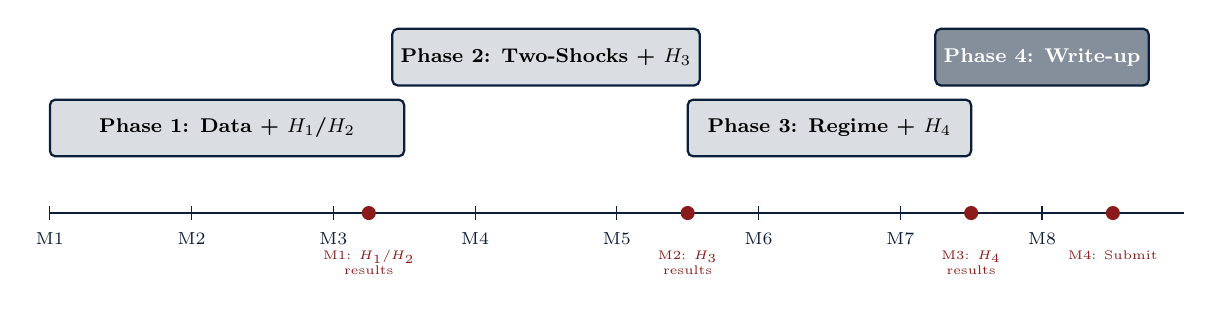
\begin{tikzpicture}[
    scale=0.9, transform shape,
    phase/.style={rectangle, rounded corners=2pt, draw=myblue, thick,
      fill=myblue!15, minimum width=3cm, minimum height=0.8cm, font=\footnotesize\bfseries, align=center},
    done/.style={phase, fill=myblue!50, text=white},
    arr/.style={-Stealth, thick, myblue!70}
  ]
    % Timeline axis
    \draw[thick, myblue] (0,0) -- (16,0);
    \foreach \x/\m in {0/M1, 2/M2, 4/M3, 6/M4, 8/M5, 10/M6, 12/M7, 14/M8} {
      \draw[myblue] (\x, -0.1) -- (\x, 0.1);
      \node[below, font=\scriptsize, text=myblue] at (\x, -0.15) {\m};
    }

    % Phase bars
    \node[phase, minimum width=5cm] (p1) at (2.5, 1.2) {Phase 1: Data + $H_1$/$H_2$};
    \node[phase, minimum width=4cm] (p2) at (7, 2.2) {Phase 2: Two-Shocks + $H_3$};
    \node[phase, minimum width=4cm] (p3) at (11, 1.2) {Phase 3: Regime + $H_4$};
    \node[done, minimum width=3cm] (p4) at (14, 2.2) {Phase 4: Write-up};

    % Milestones
    \node[circle, fill=myaccent, inner sep=2pt] (m1) at (4.5, 0) {};
    \node[circle, fill=myaccent, inner sep=2pt] (m2) at (9, 0) {};
    \node[circle, fill=myaccent, inner sep=2pt] (m3) at (13, 0) {};
    \node[circle, fill=myaccent, inner sep=2pt] (m4) at (15, 0) {};

    \node[below=0.3cm of m1, font=\tiny, text=myaccent, align=center] {M1: $H_1$/$H_2$ \\ results};
    \node[below=0.3cm of m2, font=\tiny, text=myaccent, align=center] {M2: $H_3$ \\ results};
    \node[below=0.3cm of m3, font=\tiny, text=myaccent, align=center] {M3: $H_4$ \\ results};
    \node[below=0.3cm of m4, font=\tiny, text=myaccent, align=center] {M4: Submit};
  \end{tikzpicture}
\end{frame}

\begin{frame}{Milestones \& Deliverables}
  \centering
  \footnotesize
  \begin{tabularx}{\textwidth}{l l X}
    \toprule
    \textbf{Phase} & \textbf{Timeline} & \textbf{Deliverable} \\
    \midrule
    Phase 1 & M1--M2 & Data infrastructure complete; $H_1$, $H_2$ initial results \\
    Phase 2 & M3--M4 & Two-shocks decomposition; $H_3$ results; mid-term paper draft \\
    Phase 3 & M5--M6 & Regime analysis; $H_4$ results; robustness checks \\
    Phase 4 & M7--M8 & Paper finalization; submission to \textit{JME} or \textit{JFE} \\
    \bottomrule
  \end{tabularx}

  \vspace{0.5em}
  \begin{columns}[T]
    \column{0.48\textwidth}
    \begin{ablock}{Risk Mitigation}
      \footnotesize
      \begin{itemize}
        \item WRDS access delay $\to$ fallback to FRED + yfinance
        \item FinBERT compute $\to$ cloud GPU or pre-trained
        \item Sample size concerns $\to$ bootstrap inference
      \end{itemize}
    \end{ablock}

    \column{0.48\textwidth}
    \begin{agreenblock}{Collaboration}
      \footnotesize
      \begin{itemize}
        \item \textbf{Eileen Zhang:} Economic theory, hypothesis development, writing
        \item \textbf{TA / RA:} Data pipeline, NLP implementation, empirical estimation
        \item \textbf{Advisor:} Methodological guidance, submission strategy
      \end{itemize}
    \end{agreenblock}
  \end{columns}
\end{frame}

% ========================================================================
\section{Selected References}
% ========================================================================

\begin{frame}{Selected References I}
  \footnotesize
  \begin{columns}[T]
    \column{0.48\textwidth}
    \begin{itemize}
      \item Adrian, T., \& Shin, H. S. (2010). Financial intermediaries and monetary economics. In \textit{Handbook of Monetary Economics} (Vol.~3). Elsevier.
      \item Bauer, M. D., \& Swanson, E. T. (2023). A reassessment of monetary policy surprises and high-frequency identification. \textit{NBER Macroeconomics Annual}.
      \item Bernanke, B. S., \& Kuttner, K. N. (2005). What explains the stock market's reaction to Federal Reserve policy? \textit{JFE}, 77(2).
      \item Borio, C., \& Zhu, H. (2012). Capital regulation, risk-taking and monetary policy: A missing link? \textit{J.\ Financial Stability}, 8(4).
      \item Campbell, J. R., Fisher, J. D., \& Justiniano, A. (2017). Monetary policy forward guidance. \textit{JMCB}, 49(5).
    \end{itemize}

    \column{0.48\textwidth}
    \begin{itemize}
      \item Eggertsson, G. B., \& Woodford, M. (2003). The zero bound on interest rates and optimal monetary policy. \textit{Brookings Papers on Economic Activity}, 2003(1).
      \item Froot, K. A., O'Connell, P. G. J., \& Seasholes, M. S. (2001). The portfolio flows of international investors. \textit{JFE}, 59(2).
      \item G\"urkaynak, R. S., Sack, B., \& Swanson, E. (2005). Do actions speak louder than words? \textit{IJCB}, 1(1).
      \item Jaroci\'nski, M., \& Karadi, P. (2020). Deconstructing monetary policy surprises. \textit{JME}, 115.
    \end{itemize}
  \end{columns}
\end{frame}

\begin{frame}{Selected References II}
  \footnotesize
  \begin{columns}[T]
    \column{0.48\textwidth}
    \begin{itemize}
      \item Koijen, R. S. J., \& Yogo, M. (2019). A demand system approach to asset pricing. \textit{JPE}, 127(1).
      \item Kuttner, K. N. (2001). Monetary policy surprises and interest rates. \textit{JME}, 47(3).
      \item Loughran, T., \& McDonald, B. (2011). When is a liability not a liability? \textit{JF}, 66(1).
      \item Miranda-Agrippino, S., \& Rey, H. (2020). U.S. monetary policy and the global financial cycle. \textit{RES}, 87(6).
      \item Nakamura, E., \& Steinsson, J. (2018). High-frequency identification of monetary non-neutrality. \textit{QJE}, 133(3).
    \end{itemize}

    \column{0.48\textwidth}
    \begin{itemize}
      \item Romer, C. D., \& Romer, D. H. (2000). Federal Reserve information and the behavior of interest rates. \textit{AER}, 90(3).
      \item Romer, C. D., \& Romer, D. H. (2004). A new measure of monetary shocks. \textit{AER}, 94(4).
      \item Swanson, E. T. (2021). Measuring the effects of Fed forward guidance and asset purchases. \textit{JME}, 118.
      \item Thompson, S. B. (2011). Simple formulas for standard errors that cluster by both firm and time. \textit{JFE}, 99(1).
    \end{itemize}
  \end{columns}
\end{frame}

% ── Thank you ────────────────────────────────────────────────────────────
\begin{frame}[plain]
  \vfill
  \centering
  {\Large\bfseries\color{myblue} Thank You}\\[0.5em]
  {\normalsize Questions \& Discussion Welcome}\\[1.5em]
  {\footnotesize\color{myblue!70} Eileen Zhang \quad | \quad August 2026}
  \vfill
\end{frame}

\end{document}
